\chapter{Monte-Carlo corrections}\label{chap:MCCor}
Monte Carlo plays important role in the cross-section measurement. It is constantly being improved, in order to obtain a better precision in data description. Part of these corrections have been described in Chap. \ref{chap:MC}. Unfortunately, not everything can be taken into account during simulation itself. This leads to differences between data and Monte Carlo, that need to be accounted for. There are two possible methods to correct Monte Carlo without regenerating it. First one is to apply event weights, so that each MC event can contribute by a non one entry to a histogram. This procedure is called event reweighting. Second one is a MC smearing. It uses random numbers to alter the reconstructed 4-vectors. 

This chapter describes all additional corrections, that have been applied on MC samples in this analysis. All of these correction are introducing additional systematic error, that will be discussed in the Chap. \ref{chap:Unc}.

\section{Lepton efficiency corrections}\label{sec:Eff}

The efficiency of lepton detection at \atlas detector can be divided into three components:
\begin{itemize}
\item The reconstruction efficiency $\epsilon_{rec}$ is a probability to reconstruct lepton as a lepton of this flavor.
\item The identification efficiency $\epsilon_{id \mid rec}$ is a probability that a reconstructed lepton survives  identification requirements. 
\item The trigger efficiency $\epsilon_{trig \mid rec,id}$ is a probability, that the lepton satisfies the trigger requirements. 
\end{itemize}
The full efficiency for a single lepton can be written as:
\begin{equation}
\epsilon_{total}=\epsilon_{rec} \times \epsilon_{id \mid rec} \times \epsilon_{trig \mid rec,id}
\end{equation}
All these efficiencies are measured using tag-and-probe method in $Z\to ll$ decays.  One of the leptons from Z boson, called "probe", is initially selected with all of the cuts, except the one under study. Second one, called "probe", satisfies tighter selection with some additional cut, e.g. trigger matching.

The reconstruction efficiency is associated with the algorithm used in the event reconstruction process. This is causing differences between electrons and muons efficiencies. In the electron case the reconstruction efficiency is understood as a probability to reconstruct an electron which has deposited its energy in electromagnetic calorimeter cluster as an electron candidate.  

The muon reconstruction efficiency is given by:
\begin{equation}
\epsilon_{reco,muon} = \epsilon_{reco,muon|ID} \cdot \epsilon_{ID} \approx \epsilon_{reco,muon|ID} \cdot \epsilon_{ID|MS},
\end{equation}
where $\epsilon_{reco,muon|ID}$ is a conditional probability that a muon reconstructed in ID is also reconstructed using MS as a combined muon, and  $\epsilon_{ID}$ is a probability that the muon is reconstructed as an ID track. This quantity $\epsilon_{ID}$ cannot be measured directly  in the data and therefore is replaced by $\epsilon_{ID|MS}$ - probability that muon reconstructed in MS is also reconstructed in ID, that can be measured by the tag-and-probe method. 

\begin{figure}[t]
\centering
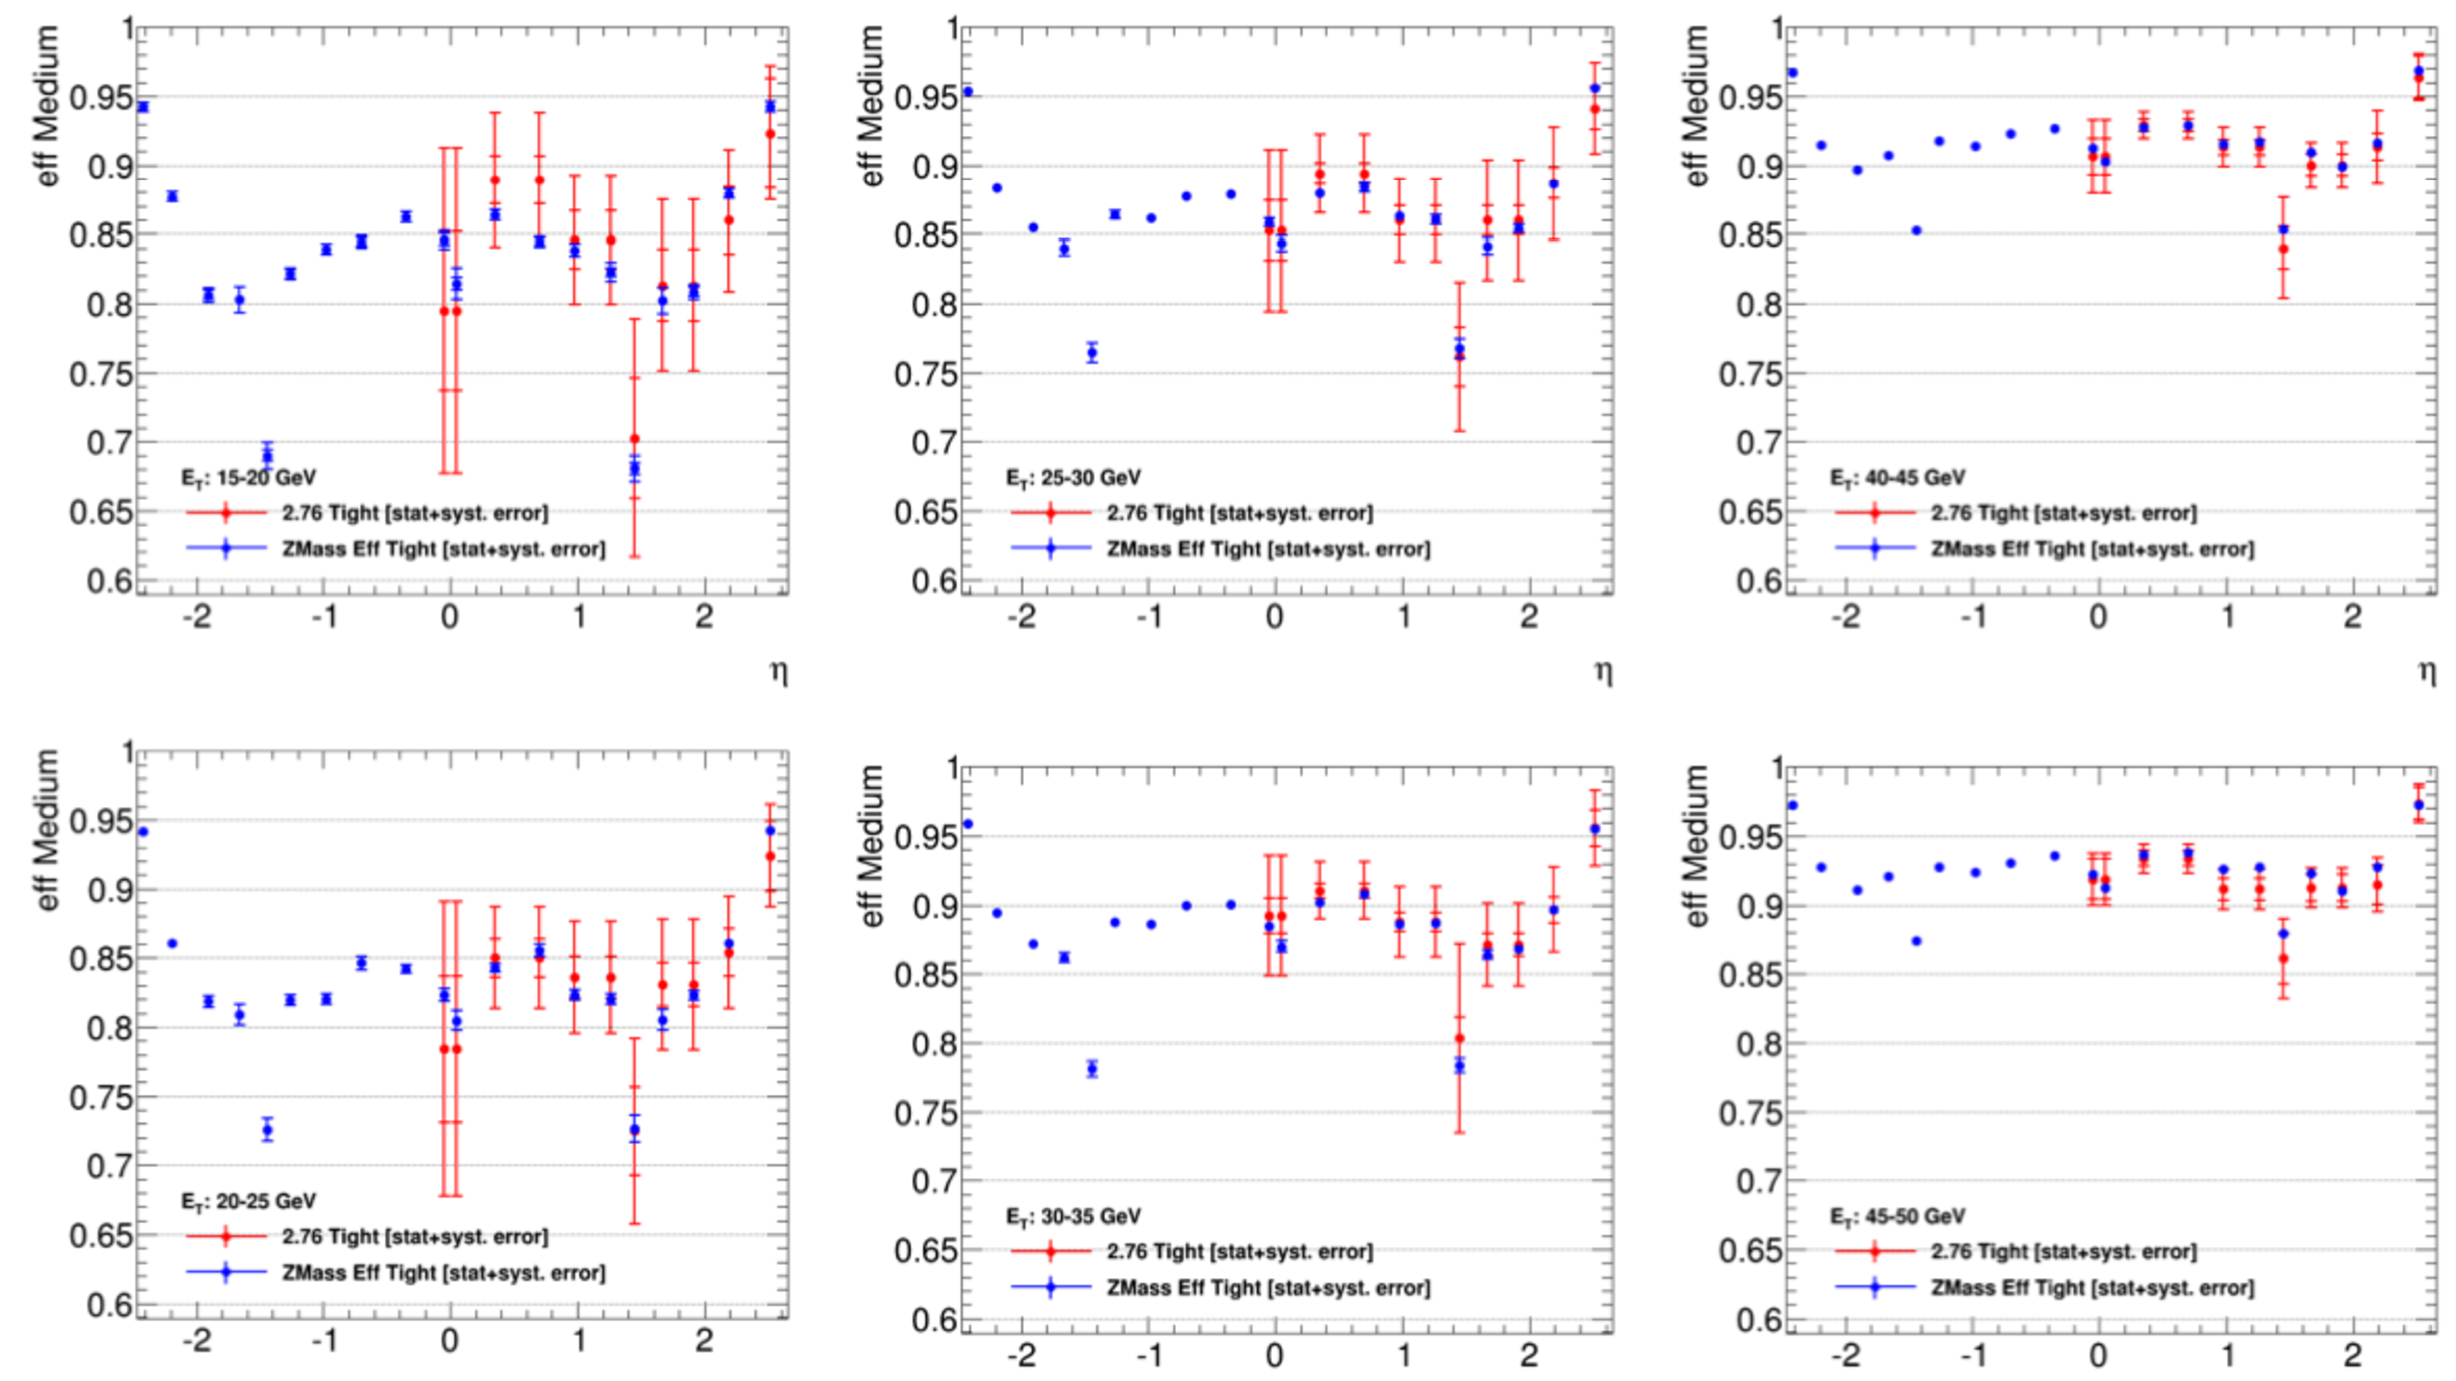
\includegraphics[width=1\textwidth]{MCCorrections/sf.pdf}
\caption{Comparition of electron efficiencies as calculated for 8TeV (blue points) and 2.76TeV (red points) for MC simulation. Efficiencies are shown as a function of pseudorapidity ($\eta$) for different electron $E_T$ bins. Both statistical and systematic uncertainties are shown. }
\label{eff_comp}
\end{figure}
Simulation samples are corrected to match data efficiencies by a scale-factor :
\begin{equation}
SF_{reco,id,trig}=\frac{\epsilon^{data}_{reco,id,trig}}{\epsilon^{MC}_{reco,id,trig}}.
\end{equation}

The scale factors are calculated in \ptl and $\eta^{l}$ bins and have associated statistical and systematic uncertainty components. The statistical component is connected to a size of $Z\to ll$, which in our case is around 500 events per each lepton flavor. This makes statistical error the dominant one and means that precise calculation of scaling factors based on this data is difficult.

It is possible, however, to use scale factors for 8 TeV 2012 data. The main difference between these data samples are center of mass energy and the pile-up conditions (10 in 2012 and less than 1 in 2013). The effects of these differences have been studied by the electron performance group at \atlas using $Z\to ee$ MC sample. Fig. \ref{eff_comp} shows the scale factors for different \ptl ranges as a function of $\eta^{l}$, for the MC data produced at 2.76TeV and 8 TeV centre-of-mass energy. The differences in the scale factors are negligible and fully covered by the statistical errors. This justifies the usage of 8 TeV scaling factors with increased uncertainty (that is considered to be fully statistical) in the analysis at 2.76 TeV. 

\subsection{Muon Trigger SF}
Unfortunatelly, single muon trigger has not been present in the 2012 data, so muon trigger scale factor had to be derived from the 2.76 TeV data. The size of the Z sample is not big enough to make the scale factors in \ptl and $\eta^{l}$ bins. 

Since the $P_{T}^{\mu}$ cut is significantly higher, than the trigger threshold, the trigger efficiency in $P_{T}^{\mu}$ can be considered flat. On the another hand, the $\eta$ dependence are expected. Binning in $\eta$ is motivated by the detector construction: $|\eta|<1.05$ corresponds to a barrel part of the muon spectrometer, while $1.05<|\eta|<2.5$ is an end-cap MS (see Sec. \ref{sec:MuonSys}). The muon trajectory is bend in a magnetic field. That can lead to small differences in a trigger efficiencies for different muon charges. Possible charge dependency of the scale factors also have been studied. 

Total scale factors are presented in Tab. \ref{tab:MuonSF}. Scale factors for $\mu^{+}$ and $\mu^{-}$ are more than 3$\sigma$ away from each other, that is a clear indicator of a charge dependency. Trigger efficiencies for data and MC in $\eta$ bins are shown in a Fig. \ref{fig:MuSF}. 

Effect of applying different scale factors on muon for W analysis is shown on Fig. ~\ref{fig:SFBined1} - ~\ref{fig:SFBined3}. Best agreement with data is achieved by applying single bin scale factor. This, toghether with the fact that difference in a efficiencies is smaller than 1$\sigma$ for most of the $\eta$ bins motivates a choice of single bin charge dependent scale factor for this analysis. 

\begin{table}[!t]
    \caption{Muon trigger scale factors}
	\label{tab:MuonSF}
	\begin{center}
		\begin{tabular}{|l | c | c|}
		\hline
		& SF & SF stat.error\\
		\hline
		\hline
		$\mu$ & 0.988 & 0.011\\
		\hline
		$\mu^{+}$ & 1.012 & 0.015\\
		$\mu^{-}$ & 0.964 & 0.015\\
		\hline
		\end{tabular}
		\end{center}
\end{table}

\begin{figure}[!b]
\minipage{0.32\textwidth}
  \center{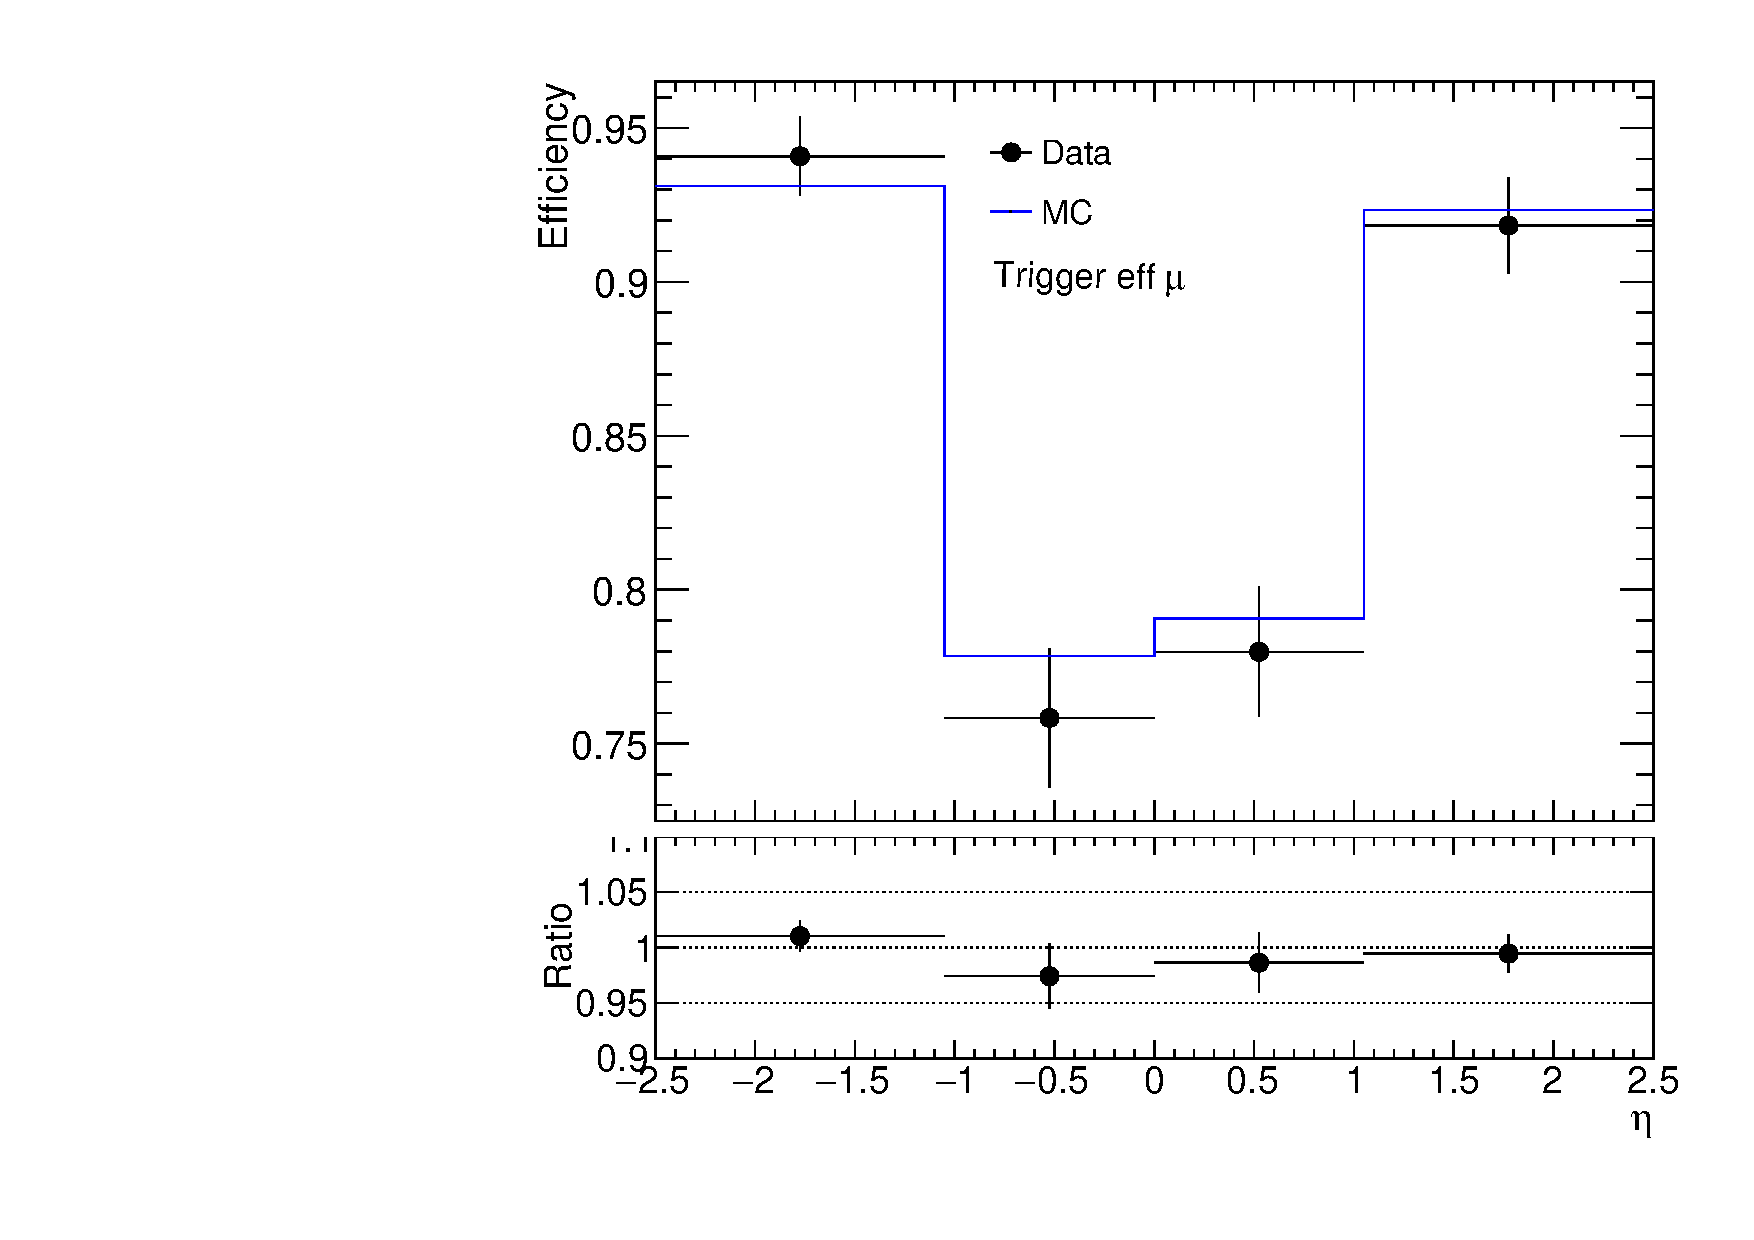
\includegraphics[width=\linewidth]{MCCorrections/m.pdf} \\ a)}
\endminipage\hfill
\minipage{0.32\textwidth}
   \center{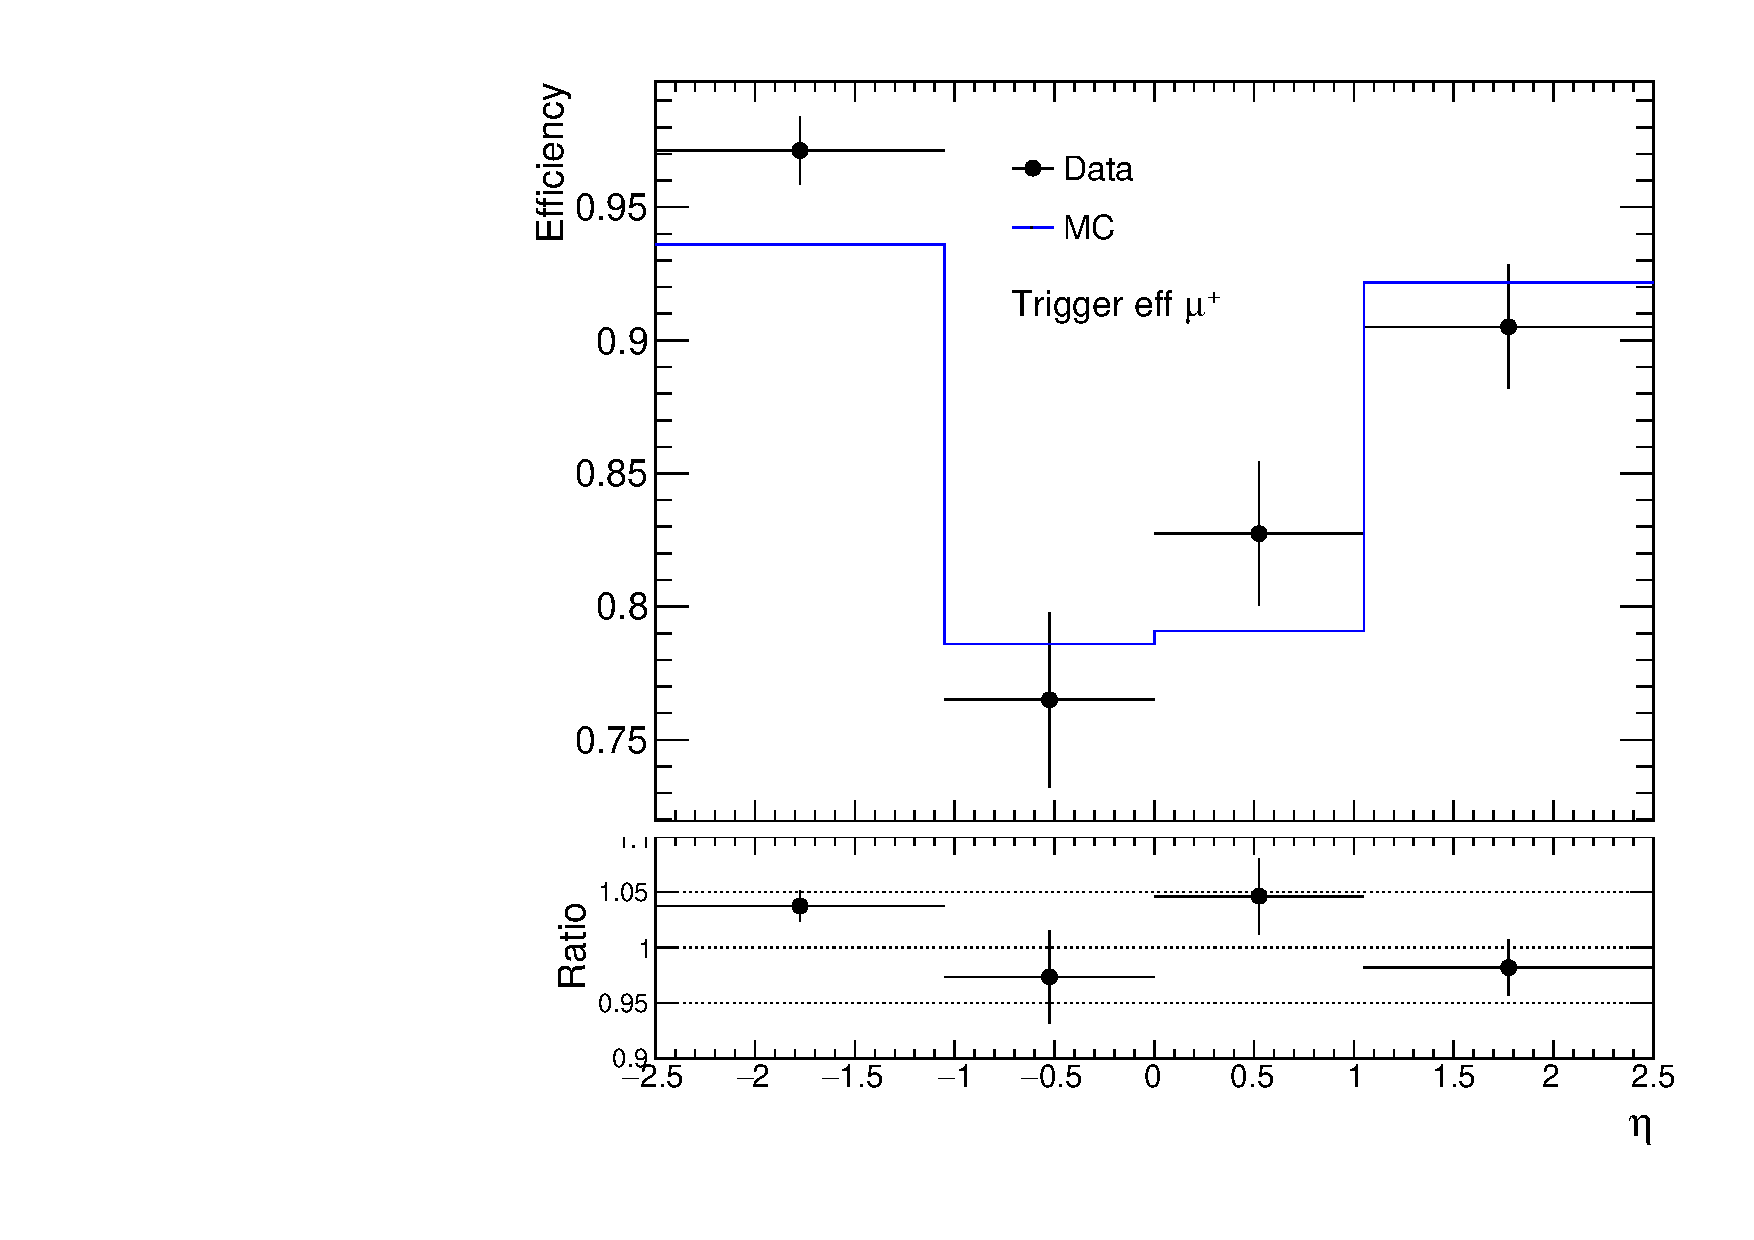
\includegraphics[width=\linewidth]{MCCorrections/mP.pdf} \\ b)}
\endminipage\hfill
\minipage{0.32\textwidth}%
   \center{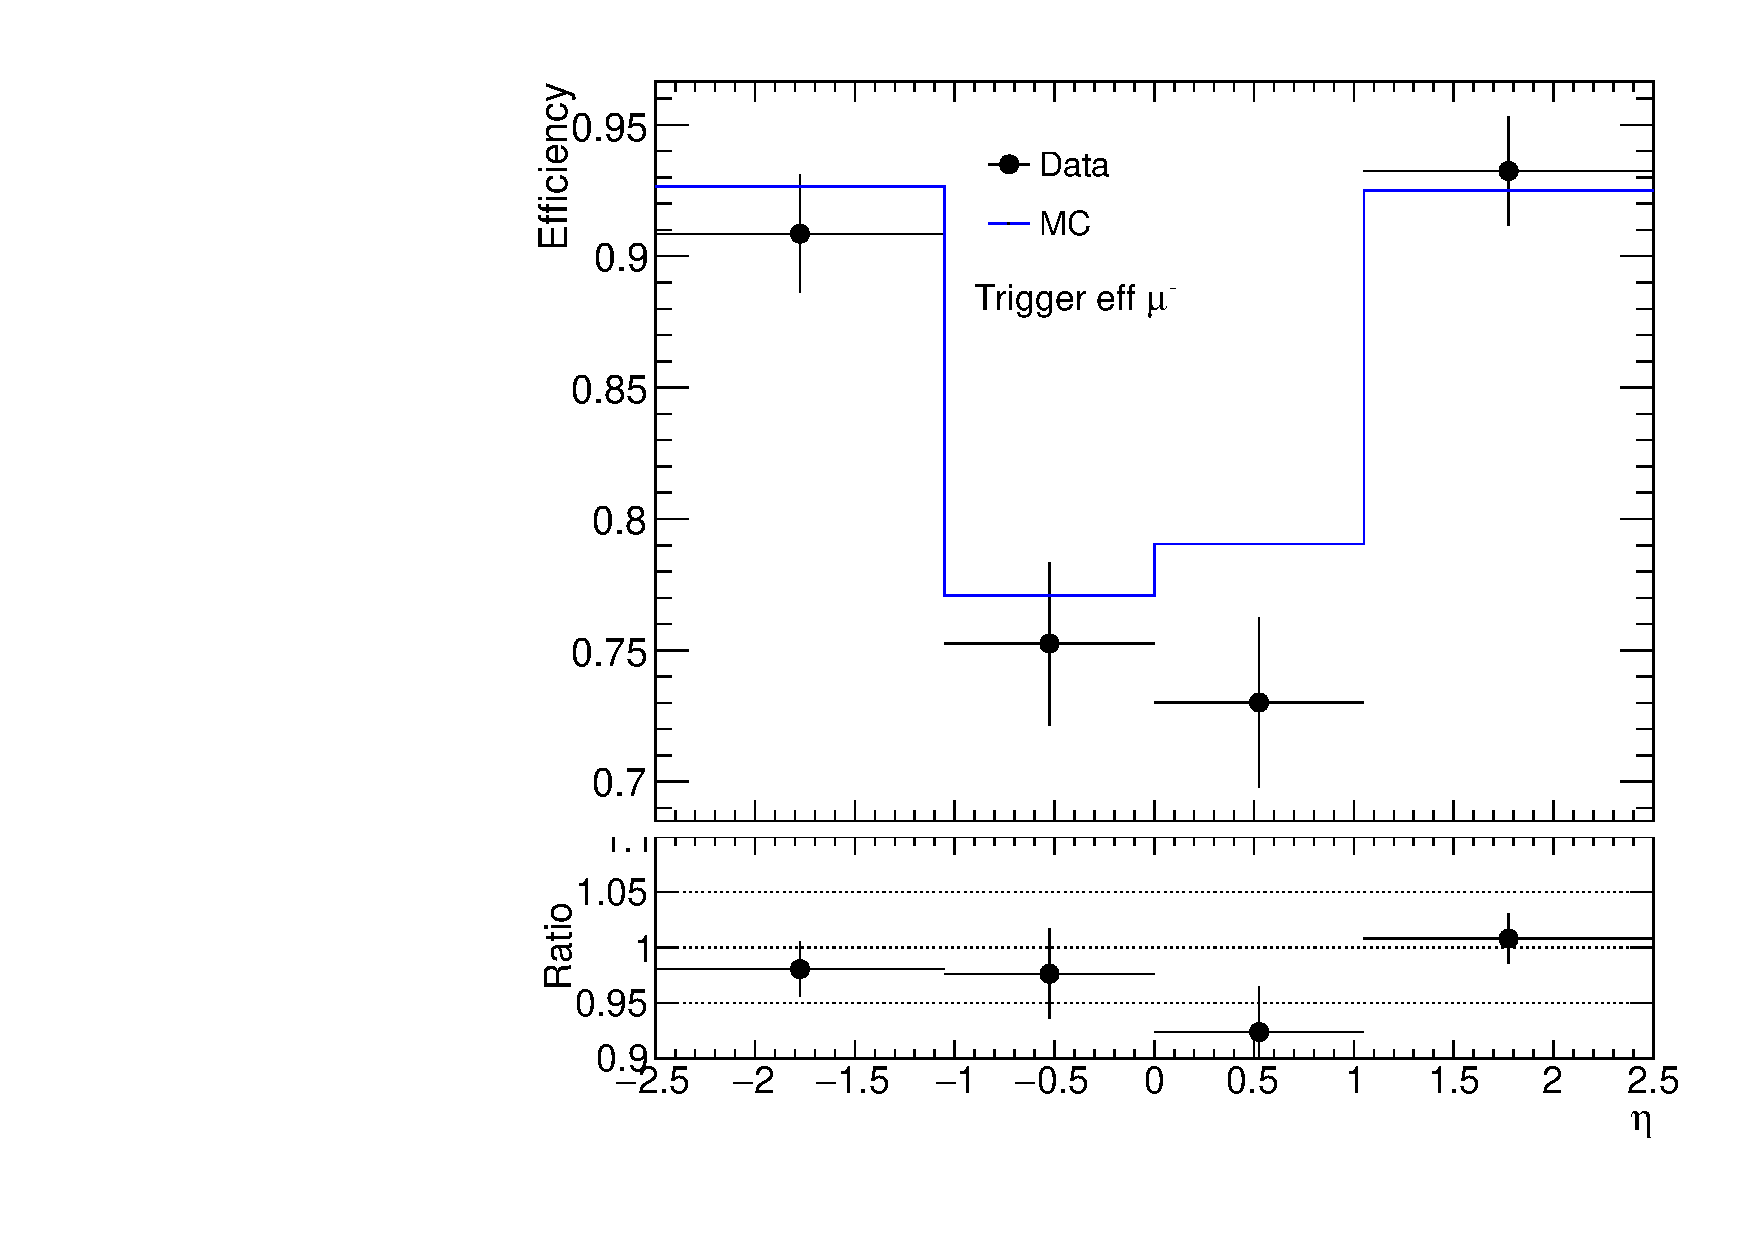
\includegraphics[width=\linewidth]{MCCorrections/mM.pdf} \\ c)}
\endminipage
\caption{Trigger scale efficiencies distribution for a) $\mu$ b) $\mu^{+}$  c) $\mu^{-}$ as a function of pseudorapidity}
\label{fig:MuSF}
\end{figure}

\begin{figure}[!tbp]
\minipage{0.5\textwidth}
  \center{\includegraphics[width=\linewidth]{MCCorrections/BinnedCharged/Wmu_Boson_lepEtaFine.pdf} \\ a)}
\endminipage\hfill
\minipage{0.5\textwidth}
  \center{\includegraphics[width=\linewidth]{MCCorrections/OneBinCharged/Wmu_Boson_lepEtaFine.pdf} \\ b)}
\endminipage\hfill
\caption{Muon pseudorapidity distribution from the $W\to \mu \nu$ selection with a) binned  b) not binned charge dependent trigger scale factor applied}
\label{fig:SFBined1}
\end{figure}

\begin{figure}[!tbp]
\minipage{0.5\textwidth}
  \center{\includegraphics[width=\linewidth]{MCCorrections/BinnedCharged/Wmu_Plus_lepEtaFine.pdf} \\ a)}
\endminipage\hfill
\minipage{0.5\textwidth}
  \center{\includegraphics[width=\linewidth]{MCCorrections/OneBinCharged/Wmu_Plus_lepEtaFine.pdf} \\ b)}
\endminipage\hfill
\caption{Muon pseudorapidity distribution from the $W\to \mu^+ \nu$ selection with a) binned  b) not binned charge dependent trigger scale factor applied}
\label{fig:SFBined2}
\end{figure}

\begin{figure}[!tbp]
\minipage{0.5\textwidth}
  \center{\includegraphics[width=\linewidth]{MCCorrections/BinnedCharged/Wmu_Minus_lepEtaFine.pdf} \\ a)}
\endminipage\hfill
\minipage{0.5\textwidth}
  \center{\includegraphics[width=\linewidth]{MCCorrections/OneBinCharged/Wmu_Minus_lepEtaFine.pdf} \\ b)}
\endminipage\hfill
\caption{Muon pseudorapidity distribution from the $W\to \mu^- \nu$ selection with a) binned  b) not binned charge dependent trigger scale factor applied}
\label{fig:SFBined3}
\end{figure}

\section{Electron energy scale and resolution}\label{sec:elecScale}
The energy of the reconstructed electron clusters tends to be shifted in comparison to the true energy of the initial electron. The correction of this shift is done in both data and MC as a 3 step procedure:
\begin{itemize}
\item Electronic calibration, that transfers a raw signal from a readout to a cluster energy deposit.
\item MC based calibration. It corrects the effects of the energy loss in the material in front of the calorimeter and the leakage into the hadronic calorimeter. This calibration is applied on both data and MC.
\item Correction of the calorimeter cell responce in the data. This allows to get the right response in non-optimal HV-regions and to exclude biases in the calorimeter electronics reconstruction.
\end{itemize}

The energy shift is parametrised, as:
\begin{equation}
E^{data}=E^{MC}(1+\alpha_i),
\end{equation}
where $E^{data}$ and $E^{MC}$ are the energies in data and simulation, respectivelly and $\alpha_i$ is a mean shift in a given bin i in $\eta$. The effect of this miscalibration on a reconstructed mass of Z boson neglecting second order terms is:
\begin{equation}
m_{i,j}^{data}=m_{i,j}^{MC}(1+\alpha_{i,j}), \quad \alpha_{i,j} \sim \frac{\alpha_i+\alpha_j}{2}, 
\end{equation}
where $m_{i,j}^{data}$ and $m_{i,j}^{MC}$ are the reconstructed mass of the Z boson in $i$ and $j$ bins in $\eta$ for data and MC respectively. 

Additionally the difference in the electron resolution has to be corrected. The dependency of electron resolution on its energy was described by Eq. \ref{eq:EMResoultion}. It is assumed, that the sampling and the noise terms are well modeled by the MC simulation and the main difference is coming from a constant term. 
So, the electron resolution correction can be written as:
\begin{equation}
\frac{\sigma_E}{E}^{Data}_{i}=\frac{\sigma_E}{E}^{MC}_{i} \oplus c_i
\end{equation}
where $c_i$ is an $\eta$ dependent relative resolution correction. Similarly to an energy scale correction it is possible to derive resolution correction factor by a comparison  of $m_{i,j}^{data}$ and $m_{i,j}^{MC}$ distributions. 

The correction values $\alpha_i$ and $c_i$are obtained via the $\chi^2$ fit of an invariant mass of electron pairs in data and MC. The resulting energy scale is applied to the data, while the resolution is corrected in MC. The resulting scale is validated using the $J/\psi \to ee$ and $Z/\gamma \to ee $ samples.

\section{Muon momentum correction}\label{sec:MuonMomCor}
The muon momentum resolution depends on $\eta$, $\phi$ and $p_T$ of the muon \cite{AtlasExperiment}. There is an empirical formula to describe it inside the detector (ID or MS):
\begin{equation}\label{eq:MuonResolution}
\frac{\sigma_{Det}(p_T)}{p_T}=\frac{r^{Det}_0(\eta, \phi)}{p_T} \oplus r^{Det}_1 (\eta, \phi)  \oplus r^{Det}_2(\eta, \phi) \cdot p_T.
\end{equation}
The first term origins from the fluctuations of the energy loss in the traversed material. The second $r^{Det}_1$ term is coming from the magnetic field inhomogenities and the local displacements. The third term $r^{Det}_2$ describes the intrinsic resolution effects. 

Similarly to electrons, the overall energy scale shift between data and MC is parameterised as:
\begin{equation}
p_T^{data}=p_T^{MC}+s_0^{Det}(\eta, \phi)+s_1^{Det}(\eta, \phi) \cdot p_T^{MC},
\end{equation}
where $s_0^{Det}(\eta, \phi)$ is coming from the imperfect knowledge of energy losses for muons passing through detector. 

This leads to a total correction formula:
\begin{equation}
p^{Cor,Det}_T=\frac{p_{T}^{MC,Det}+\sum\limits_{n=0}^1 s_n^{Det}(\eta, \phi)(p_T^{MC,Det})^n}{1+\sum\limits_{m=0}^2 \Delta r_m^{Det}(\eta, \phi)(p_T^{MC,Det})^{m-1} g_m},
\end{equation}
where $g_m$ are normally distributed random variables with the mean 0 and the width 1. Due to a small amount of material between the interaction point and the ID, $\Delta r^{ID}_0(\eta, \phi)$ and $s_0^{ID}(\eta, \phi)$ are set to 0. The misalignment effect of the MS is corrected on a simulation level by adding a random smearing to the alignment constants. This allows to set $\Delta r^{MS}_2(\eta, \phi)$ to 0 during the fit. 

The correction factors are extracted using events with $Z \to \mu \mu$, where muon candidates fulfill the combined muon criteria described in Sec.\ref{sec:MuonRec}. For the correction, the invariant mass distributions $m_{\mu\mu}^{ID}$ and $m_{\mu\mu}^{MS}$ are considered individually within a specific $\eta - \phi$ region of the fit. The combined muon parameters are used to obtain angles $\eta$ and $\phi$. 
The correction extraction is performed first for the ID and then for the MS. Additionally, the following fit variable is considered:
\begin{equation}
\rho = \frac{p_T^{MS}-p_T^{ID}}{p_T^{ID}},
\end{equation}
which represents the $p_T$ imbalance between the ID and the MS. 

In a second step corrections are propagated to the combined momentum, using a weight average:
\begin{equation}
p_T^{Cor,CB}= f\cdot p_T^{Cor,ID}+(1-f) \cdot p_T^{Cor,MS},
\end{equation}
where the weight f is derived from the MC. 
